
\documentclass[12pt,a4paper]{article}

% ---------- Packages ----------
\usepackage[utf8]{inputenc}
\usepackage[T1]{fontenc}
\usepackage{lmodern}
\usepackage[margin=2.5cm]{geometry}
\usepackage{setspace}
\doublespacing
\usepackage{lineno}
\linenumbers
\usepackage{graphicx}
\usepackage{booktabs}
\usepackage{tabularx}
\usepackage{longtable}
\usepackage{array}
\usepackage{multirow}
\usepackage{amsmath,amssymb}
\usepackage{xcolor}
\usepackage{enumitem}
\usepackage{caption}
\usepackage{subcaption}
\usepackage{float}
\usepackage{listings}
\usepackage{url}
\usepackage{xurl}
\usepackage{seqsplit}

\newcolumntype{Y}{>{\setstretch{1.15}\selectfont\raggedright\arraybackslash}X}
\newcolumntype{Z}{>{\setstretch{1.05}\selectfont\raggedright\arraybackslash}X}
\newcolumntype{P}[1]{>{\raggedright\arraybackslash}p{#1}}
\usepackage[colorlinks=true,linkcolor=blue,citecolor=blue,urlcolor=blue]{hyperref}
\usepackage[round,authoryear]{natbib}

% ---------- Path formatting note ----------
% Use \texttt{...} for short file and folder names; escape underscores as \_.
% Avoid escaped underscores inside \path{...}.

% ---------- Formatting ----------
\setlength{\parskip}{0.25em}
\setlength{\parindent}{1.2em}
\renewcommand{\arraystretch}{1.15}
\emergencystretch=3em
% Improve line breaking for long paths and URLs
\Urlmuskip=0mu plus 1mu\relax


% ---------- TODO command ----------
\newcommand{\todo}[1]{\textcolor{red}{\textbf{[TODO: #1]}}}

% ---------- Listing style ----------
\lstdefinestyle{hydrocode}{
  basicstyle=\small\ttfamily,
  breaklines=true,
  frame=single,
  backgroundcolor=\color{gray!8},
  showstringspaces=false,
  numbers=left,
  numberstyle=\tiny\color{gray},
  numbersep=5pt,
  tabsize=2,
  columns=fullflexible,
  keepspaces=true,
  breakatwhitespace=false,
  postbreak=\mbox{\textcolor{gray}{$\hookrightarrow$}\space}
}
\lstset{style=hydrocode}

% ---------- Placeholder figure ----------
\newcommand{\placeholderfigure}[2]{%
\begin{figure}[H]
\centering
\fbox{%
\begin{minipage}[c][0.22\textheight][c]{0.88\textwidth}
\centering
\textbf{#1}\\[0.5em]
#2
\end{minipage}}
\caption{#1}
\end{figure}}

% ============================================================
\begin{document}

\begin{flushleft}
{\LARGE\bfseries HydroAgent: A Framework-Agnostic Conversational Agent for Hydrological Workflow Planning and Execution}
\end{flushleft}

\vspace{0.6em}

\begin{flushleft}
Ali Akbar Jamali$^{1}$, Raymond J Spiteri$^{1,*}$\\[0.4em]

$^{1}$Department of Computer Science, University of Saskatchewan, Saskatoon, Canada\\
$^{*}$Corresponding author: \href {mailto:spiteri@cs.usask.ca}{spiteri@cs.usask.ca}
\end{flushleft}

\vspace{0.5em}
\hrule
\vspace{1em}

% ============================================================
\section*{Graphical abstract}
% ============================================================


% ============================================================
\section*{Highlights}
% ============================================================

\begin{itemize}[leftmargin=*,noitemsep]
  \item HydroAgent translates natural-language hydrological modelling requests into 
  structured, backend-independent workflow plans.
  \item A hybrid design combines LLM planning with deterministic schemas, operation 
  catalogs, validation rules, and explicit execution gates.
  \item A backend-adapter layer separates general workflow planning from framework-specific 
  configuration generation and execution.
  \item The Streamlit interface integrates prompt-based planning, conversational refinement, 
  map-based spatial input, configuration preview, and live execution logs.
  \item Bow River at Banff case studies demonstrate cloud-from-scratch execution, dependency 
  handling, local-artifact reuse, and conversational plan refinement using SYMFLUENCE as the 
  first backend.
  \item A 25-prompt evaluation across OpenAI, Gemini, and Claude showed reliable core-field 
  extraction but provider-specific differences in step selection, missing-input handling, and 
  negative-constraint compliance.\end{itemize}

% ============================================================
\begin{abstract}  
% ============================================================
Integrated hydrological modelling frameworks are powerful but configuration-heavy, 
requiring users to manage spatial domains, forcing and observational data, model-specific 
inputs, workflow dependencies, and execution settings. This paper presents HydroAgent, 
a large language model (LLM)-assisted workflow agent for planning, configuring, and 
executing hydrological modelling workflows. HydroAgent uses a framework-agnostic 
architecture in which natural-language requests are converted into structured JSON 
workflow plans, validated against an operation catalog, mapped through a backend-specific 
configuration adapter, and executed through controlled workflow steps. In this study, 
SYMFLUENCE is used as the first backend implementation and case-study platform.

HydroAgent combines a Streamlit interface, a multi-provider LLM layer, deterministic 
plan-repair rules, parameter registries, explicit execution gates, and interactive 
spatial input. We demonstrate the system using Bow River at Banff workflows, including 
a cloud-from-scratch semi-distributed SUMMA--mizuRoute run, a lumped SUMMA workflow 
with automatically added routing, a local-artifact reuse workflow, and a conversational 
refinement case. The completed case studies show that HydroAgent can generate executable 
workflow plans, preserve run-level provenance artifacts, reuse existing domain and forcing 
data, regenerate stale preprocessing/model files, and complete SUMMA and mizuRoute execution. 
The semi-distributed and lumped cases produced non-empty SUMMA outputs with 35,063 timestep 
records and 1,460 daily records.

A 25-prompt prompt-to-plan evaluation was conducted across OpenAI, Google Gemini, and 
Anthropic Claude. All three providers generated usable structured plans for most prompts 
and generally extracted core configuration fields correctly, but they differed in planning 
style: OpenAI was more conservative, Gemini more often preserved specialized configuration 
details, and Claude produced more detailed but often more expansive workflow plans. These 
results support HydroAgent's provider-agnostic design, in which LLM outputs are treated as 
draft plans requiring schema validation, dependency repair, and explicit execution gating 
before backend execution. The lumped case also revealed a limitation: routing was automatically 
added despite the prompt requesting a SUMMA-only workflow, highlighting the need to keep 
generated plans, dependency resolution, and execution logs visible to users.
\end{abstract}

\noindent\textbf{Keywords:} hydroinformatics; large language models; hydrological modelling; 
workflow automation; framework-agnostic agents; SYMFLUENCE; SUMMA; mizuRoute; scientific agents

% ============================================================
\section{Introduction}
\label{sec:introduction}
% ============================================================

Process-based hydrological modelling depends on integrated workflows that combine spatial 
domain definition, forcing acquisition, observation processing, numerical simulation, 
routing, calibration, and post-processing. Frameworks such as SUMMA \citep{clark2015b, clark2015a, clark2021}, 
FUSE \citep{clark2008}, and mizuRoute \citep{mizukami2016} provide flexible representations 
of hydrological processes and routing, while orchestration frameworks such as SYMFLUENCE aim to connect data services, 
hydrological models, routing components, calibration routines, and evaluation tools across complete experiments \todo{add SYMFLUENCE citation}. 
However, this flexibility comes with a substantial operational burden. Users must select the 
correct workflow steps, prepare geospatial inputs, configure forcing datasets, specify time 
periods, define calibration settings, and maintain consistent file paths and naming conventions.

This complexity creates a gap between hydrological expertise and computational execution of 
hydrological models. Domain scientists may understand the basin, model assumptions, and 
desired experiment, but still have difficulty in translating that intent into a valid 
configuration file and executable workflow. Conversely, software specialists may understand 
the principles of running a framework but lack the hydrological knowledge needed to choose 
proper options. In tutorial notebooks, many of these decisions are hidden in prewritten 
cells; however, outside tutorials, users must reconstruct them manually.

Large language models (LLMs) offer a promising interface layer for scientific computing because 
they can translate natural-language goals into structured computational artifacts, including 
code, configuration files, and execution plans \citep{yildiz2025,culver2024}. However, 
relying on free-text generation alone is not enough for hydrological modelling. For example, 
an LLM may hallucinate parameter values, miss required workflow dependencies, or suggest 
execution steps that are inappropriate or unsafe \citep{agarwal2024,wang2024}. 
HydroAgent addresses this limitation through a hybrid architecture in which the LLM generates 
an initial workflow plan, and deterministic rules, operation catalogs, parameter registries, 
and validation checks constrain, correct, and validate the plan before execution.

This paper introduces HydroAgent, a framework-agnostic conversational workflow agent for 
hydrological modelling. HydroAgent separates the agent layer from the modelling-framework layer: 
the agent layer handles natural-language interaction, structured planning, validation, refinement, 
and execution gating, while backend adapters translate validated plans into framework-specific 
configuration files and execution commands. In the current implementation, SYMFLUENCE is used as 
the first backend adapter and case-study platform. The agent is designed around the principle that 
the plan, not the raw LLM response, should be reliable. User requests are converted into a structured 
JSON plan containing configuration parameters, workflow steps, missing inputs, and notes. The plan 
is displayed to the user, can be edited through both forms and chat, and is converted into a 
backend-compatible configuration file. For the SYMFLUENCE case study, this file is a reproducible 
\texttt{config.yaml}. Dangerous steps such as \texttt{run\_model} and \texttt{calibrate\_model} require 
explicit user confirmation before execution.

The contributions of this paper are:
\begin{enumerate}[leftmargin=*,noitemsep]
  \item A framework-agnostic agent architecture for translating natural-language hydrological 
  modelling requests into structured workflow plans.
  \item A hybrid planning approach that combines LLM-generated plans with deterministic schemas, 
  operation catalogs, dependency repair, parameter registries, and validation checks.
  \item A backend-adapter design that separates general workflow planning from framework-specific 
  configuration generation and execution.
  \item A Streamlit-based interface for spatial input, prompt-based planning, conversational 
  refinement, configuration preview, execution logs, and reproducible run management.
  \item A SYMFLUENCE-based case study demonstrating the architecture on executable Bow River at 
  Banff hydrological modelling workflows.
  \item A 25-prompt prompt-to-plan evaluation and three-provider comparison showing that OpenAI, 
  Gemini, and Claude produce usable structured workflow drafts, but differ in conservativeness, 
  specialized configuration extraction, and workflow-step expansion.
\end{enumerate}

The remainder of this paper is organized as follows. Section~\ref{sec:background} reviews related 
work. Section~\ref{sec:architecture} describes the system architecture. Section~\ref{sec:implementation} 
presents implementation details. Section~\ref{sec:casestudies} describes the case studies. 
Section~\ref{sec:evaluation} presents the prompt-to-plan evaluation, provider comparison, 
negative-constraint analysis, and case-study execution outcomes. Sections~\ref{sec:discussion} 
and~\ref{sec:conclusions} discuss implications, limitations, and conclusions.


\section{Background and related work}
\label{sec:background}

\subsection{Integrated hydrological modelling frameworks}

Modern hydrological modelling uses modular frameworks that separate process representation, 
numerical solution, geospatial preprocessing, routing, and evaluation. SUMMA was designed 
to provide a unified framework for testing multiple modelling alternatives, allowing users 
to combine process parameterizations and numerical methods in a controlled way \citep{clark2015b,clark2015a}. 
mizuRoute provides network routing capabilities that can be coupled to land-surface and hydrological 
model outputs \citep{mizukami2016}. Workflow orchestration frameworks such as SYMFLUENCE build on 
this ecosystem by connecting domain setup, forcing acquisition, preprocessing, model execution, 
routing, calibration, and evaluation. In this paper, SYMFLUENCE is treated as a representative 
hydrological modelling backend for demonstrating HydroAgent's backend-adapter design. \todo{Add the exact SYMFLUENCE citation}

These models improve reproducibility and flexibility, however, they also introduce complex 
dependencies. For example, a semi-distributed SUMMA run may require a DEM-derived domain, 
HRU/GRU shapefiles, catchment--forcing intersections, model-specific NetCDF inputs, routing 
topology files, and observational streamflow records. A missing or misordered step can produce 
errors that are difficult for new users to interpret.

\subsection{Scientific workflow systems}

General workflows such as Snakemake and the Common Workflow Language provide mechanisms for 
dependency tracking, rule-based execution, and reproducible computational pipelines \citep{koster2012,crusoe2022}. 
These systems are powerful but usually require users to write formal workflow definitions. 
HydroAgent addresses a different interaction model: the user states an experiment goal in 
natural language, the agent proposes a structured workflow plan, and deterministic rules validate the 
plan against a backend-specific operation catalog. Thus, HydroAgent is designed to complement formal 
workflow tools rather than replace them.

\subsection{Hydrological interfaces and decision-support systems}

Graphical interfaces for hydrological modelling, including GIS-based model setup tools and 
domain-specific decision-support systems, have long aimed to reduce the technical burden of 
model configuration \citep{tsegaye2024, xiang2023}. These interfaces typically expose 
model-specific forms, maps, and file selectors. However, most are rigid: they support a 
fixed set of workflows and require manual navigation through the interface. HydroAgent 
instead treats the interface as a conversational planning surface. Users can describe a 
target experiment, inspect the generated plan, refine it through chat, and execute selected steps.

\subsection{LLM agents for scientific computing}

LLM agents combine language understanding with tool use, structured output, and multi-step 
planning. In scientific computing, this pattern can be used to translate user intent 
into executable code, configuration files, or workflow steps \citep{li2024,ruan2023}. 
However, scientific workflows require more than plausible text. HydroAgent treats the 
LLM as one component in a controlled workflow system. Schemas, operation catalogs, validation 
checks, backend adapters, and human-in-the-loop execution gates constrain and verify 
model-generated outputs before execution.

\section{System architecture and design}
\label{sec:architecture}

\subsection{Overall architecture}

HydroAgent is organized as a four-layer architecture, as shown in Figure~\ref{fig:architecture}: 
(i) a presentation layer, (ii) a planning layer, (iii) an orchestration layer, and 
(iv) an execution layer. The presentation layer collects natural-language prompts, 
structured form inputs, spatial map selections, voice input, and chat refinements. 
The planning layer converts user requests into a structured JSON workflow plan using 
provider-specific adapters for OpenAI, Google Gemini, and Anthropic models while 
maintaining a shared plan schema. The orchestration layer validates and repairs the 
generated plan, resolves workflow dependencies, and passes the normalized specification to a 
backend adapter. Finally, the execution layer runs approved backend workflow steps, streams logs 
to the interface, and preserves run artifacts for reproducibility. In the implementation evaluated 
here, the backend adapter targets SYMFLUENCE by generating a \texttt{config.yaml} file and invoking 
SYMFLUENCE workflow steps.

\begin{figure}[!t]
  \centering
  \includegraphics[width=\textwidth]{figs/architecture.png}
  \caption{System architecture of HydroAgent. The framework is organised into four 
  layers: (1) the Presentation layer provides a Streamlit-based web interface, an 
  interactive Folium map for pour-point and bounding-box selection, and voice 
  transcription via OpenAI Whisper or Google Gemini; (2) the Planning layer translates 
  natural-language requests into structured workflow plans using one of three 
  interchangeable LLM backends (GPT, Gemini, or Claude), enforcing a shared JSON schema 
  and supporting iterative refinement through a conversational chat interface; 
  (3) the Orchestration layer resolves step dependencies against an operation catalog, 
  synthesises a backend-compatible configuration file through a parameter registry and backend adapter, and 
  validates the resulting plan; and (4) the Execution layer invokes the selected hydrological modelling backend as a 
  managed subprocess, streams live model output to the UI, and persists all run 
  artefacts including \texttt{plan.json}, backend configuration files, and \texttt{chat.json} to 
  a versioned run folder.}
  \label{fig:architecture}
\end{figure}


\subsection{Workflow representation}

The central internal representation is a JSON plan with four top-level fields: \texttt{config}, 
\texttt{steps}, \texttt{needs\_user\_input}, and \texttt{notes}. The \texttt{config} object 
contains canonical parameters such as \texttt{domain\_name}, \texttt{experiment\_id}, 
\texttt{pour\_point\_coords}, \texttt{hydrological\_model}, \texttt{forcing\_dataset}, 
\texttt{data\_access}, and calibration settings. The \texttt{steps} array defines the intended 
workflow. The \texttt{needs\_user\_input} array prevents execution when required inputs 
are missing. The \texttt{notes} field records assumptions and planner decisions.

\clearpage
{\linespread{0.9}\selectfont
\begin{lstlisting}[caption={Simplified JSON plan schema used by HydroAgent.},label={lst:plan-schema}]
{
  "config": {
    "domain_name": "Bow_at_Banff_semi_distributed",
    "experiment_id": "run_1",
    "pour_point_coords": "51.1722/-115.5717",
    "bounding_box_coords": "51.68/-116.70/50.86/-115.24",
    "hydrological_model": "SUMMA",
    "routing_model": "mizuRoute",
    "forcing_dataset": "ERA5",
    "data_access": "CLOUD"
  },
  "steps": [
    "validate_config",
    "setup_project",
    "create_pour_point",
    "acquire_attributes",
    "define_domain",
    "discretize_domain",
    "acquire_forcings",
    "process_observed_data",
    "model_agnostic_preprocessing",
    "model_specific_preprocessing",
    "run_model",
    "postprocess_results"
  ],
  "needs_user_input": [],
  "notes": "Cloud-from-scratch semi-distributed SUMMA workflow."
}
\end{lstlisting}
}

\subsection{Operation catalog and dependency resolution}

HydroAgent uses an operation catalog to describe backend workflow steps, their prerequisites, 
and whether they are safe, dangerous, proven, or experimental. The dependency resolver checks 
the LLM-generated plan against this catalog. If a user asks to run a model but omits preprocessing, 
the resolver can insert required steps or block execution with a missing-input message. The same 
mechanism distinguishes cloud-from-scratch workflows from local-data reuse workflows. For example, 
a local-data workflow may intentionally skip data-acquisition steps, whereas a cloud-from-scratch 
workflow should include them. In the current case-study implementation, the operation catalog is 
written for SYMFLUENCE workflow steps.

\subsection{Config generation and validation}

As shown in Figure~\ref{fig:plan-to-config}, HydroAgent transforms a natural-language request 
into a backend-specific model configuration through a staged plan-to-configuration workflow. 
First, the user prompt is converted by the LLM into a structured JSON plan containing the 
requested model settings, domain information, and workflow steps. The plan is then passed 
through a dependency-repair stage, where step ordering and missing prerequisites are checked 
against the operation catalog. Next, the repaired plan is translated into an intermediate 
YAML specification by mapping user-facing parameters to the fields expected by the selected backend. 
Finally, a backend adapter writes the executable configuration file. In the SYMFLUENCE case study, 
this output is a backend-compatible \texttt{config.yaml} file.

\begin{figure}[!t]
  \centering
  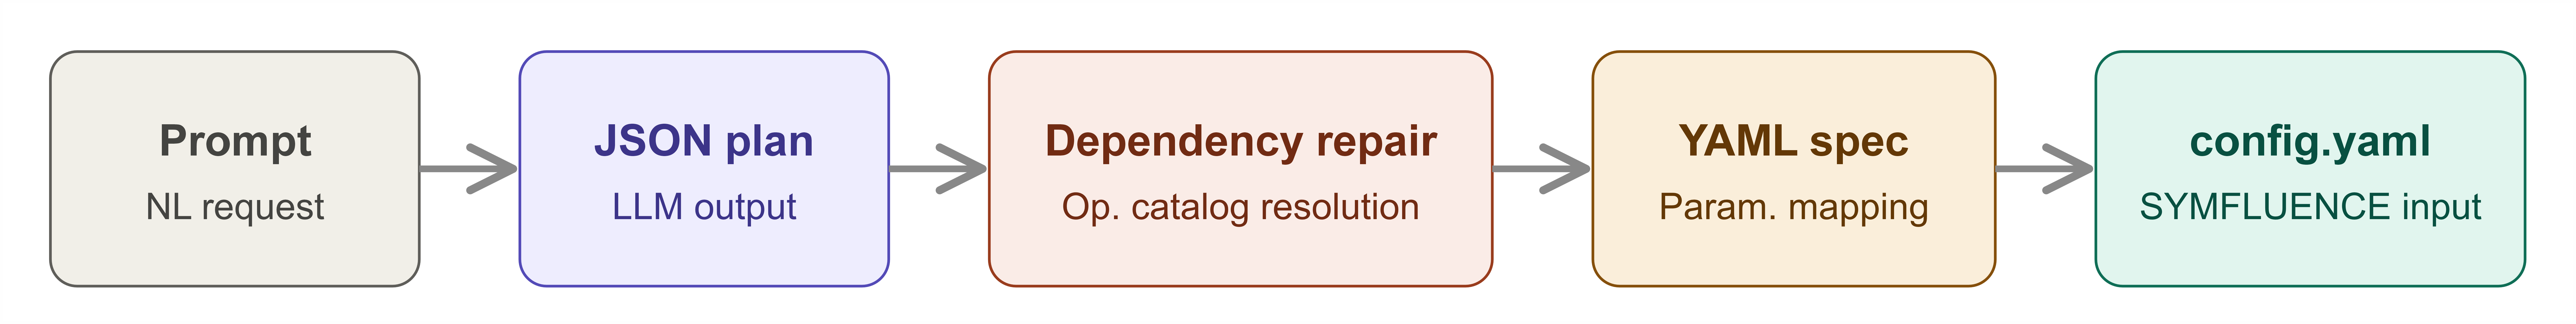
\includegraphics[width=\textwidth]{figs/plan_to_config_workflow.png}
  \caption{Plan-to-configuration workflow in HydroAgent. A natural-language prompt is converted 
  into a structured JSON plan, repaired using operation-catalog dependencies, mapped into a 
  YAML specification, and finally written as a backend-specific configuration file. In the case study, 
  the backend-specific output is a SYMFLUENCE \texttt{config.yaml} file for execution.}
  \label{fig:plan-to-config}
\end{figure}

\subsection{Conversational refinement}

After initial planning, users can refine the plan through a chat interface. HydroAgent passes the 
current plan, selected run context, and user message to a refinement prompt. Deterministic rules 
are applied before and after the LLM call for common edits such as changing dates, forcing datasets, 
model names, or step lists. The revised plan is synchronized with the UI forms and configuration 
preview. Chat history is saved with the run so that the reasoning path leading to a final configuration 
can be audited.

\subsection{Spatial input and visualization}

A Folium-based map allows the user to select or confirm pour points and bounding boxes interactively. 
These values are synchronized with the planning form and plan JSON. After domain generation, map 
layers can be used to inspect pour points, river basins, river networks, and HRU/GRU shapefiles. 
This spatial review step is particularly important because small errors in coordinates or bounding 
boxes can produce incorrect basin delineations.

\subsection{Safety controls}

HydroAgent separates planning from execution. Safe steps such as \texttt{validate\_config} and 
\texttt{setup\_project} can be executed directly, whereas dangerous or expensive steps such as 
\texttt{run\_model}, \texttt{calibrate\_model}, and large cloud downloads require explicit user 
confirmation. The UI presents the plan and configuration preview before execution and writes an 
execution log as each step runs.

% ============================================================
\section{Implementation}
\label{sec:implementation}
% ============================================================

\subsection{Software stack}

HydroAgent is implemented in Python with a Streamlit front-end. It uses GeoPandas and Folium for 
geospatial display, provider SDKs for LLM calls, and YAML and JSON utilities for plan and 
configuration generation. The core interface, planning logic, validation rules, and run-management 
components are separated from backend-specific execution. For the experiments reported in this 
paper, HydroAgent is installed alongside a SYMFLUENCE repository and data directory, and a 
SYMFLUENCE adapter invokes its command-line step execution interface.

\subsection{Run persistence}

Each HydroAgent run is stored in a dedicated folder under \texttt{runs/}. The run folder 
includes \texttt{prompt.txt}, \texttt{plan.json}, a backend configuration file, \texttt{spec.json}, 
\texttt{chat.json}, and an execution log. For the SYMFLUENCE backend, the configuration 
file is \texttt{config.yaml} and large model artifacts are written under \path{SYMFLUENCE_data/domain_*}. 
This separation allows a user to reproduce the exact plan and configuration even if large 
model outputs are stored elsewhere.

{
\renewcommand{\arraystretch}{0.8}

\begin{table}[H]
\centering
\caption{Representative HydroAgent artifacts saved for each run.}
\label{tab:artifacts}
\begin{tabularx}{\textwidth}{lY}
\toprule
\textbf{Artifact} & \textbf{Purpose} \\
\midrule
\texttt{prompt.txt} & Original natural-language request submitted by the user to create 
the run. \\
\texttt{plan.json} & Structured workflow plan generated or refined from natural language. \\
\texttt{config.yaml} & Backend-compatible configuration used for execution; in the case 
study, this is the SYMFLUENCE configuration file. \\
\texttt{spec.json} & Intermediate normalized specification used to build the YAML file. \\
\texttt{chat.json} & Conversational refinements and user decisions. \\
\texttt{logs/execution.log} & Step commands, return codes, and execution output. \\
\path{SYMFLUENCE_data/domain_*} & Backend output directory for domain, forcing, settings, 
simulation, calibration, and reporting artifacts in the SYMFLUENCE case study. \\
\bottomrule
\end{tabularx}
\end{table}
}

\subsection{Multi-provider LLM layer}

HydroAgent exposes a common interface for multiple large language model (LLM) providers. 
Provider adapters transform the shared planner prompt into provider-specific API calls 
and parse the returned JSON responses. The current implementation supports three providers: 
\href{https://developers.openai.com/api/reference/overview/}{OpenAI} for the GPT model family, 
\href{https://ai.google.dev/gemini-api/docs}{Google Gemini}, and 
\href{https://platform.claude.com/docs/en/home}{Anthropic Claude}. This multi-provider design 
allows users to switch providers and models from the workflow interface without changing downstream 
plan normalization, configuration generation, or SYMFLUENCE execution. It also supports 
institutional flexibility, controlled cost and performance comparisons, and robustness to 
provider-specific outages or service limitations \citep{openai_api_docs,google_gemini_api_docs,anthropic_claude_api_docs}.

Unless otherwise noted, the executable case studies reported here used OpenAI
\texttt{gpt-5-mini} as the default planner model. The same 25-prompt planning set was also 
evaluated with Google \texttt{gemini-2.5-flash} and Anthropic 
\texttt{claude-sonnet-4-20250514}. The three providers produced broadly usable structured 
plans, but their planning behavior differed. OpenAI was generally more conservative, Gemini 
more often preserved specialized configuration details, and Claude produced more detailed but 
often more expansive workflow plans. HydroAgent therefore treats provider outputs as draft 
plans that must pass through shared schema validation, deterministic normalization, dependency 
repair, and execution gating before backend execution.

\subsection{Local-data and cloud-data pathways}

A key implementation challenge for any backend adapter is distinguishing local-data reuse 
from cloud-from-scratch execution. In local-data reuse, previously prepared attributes, forcings, 
observations, and catchment-intersection files are intentionally reused. In cloud-from-scratch 
execution, these artifacts must be regenerated in the correct order. HydroAgent therefore records 
data-access intent in the plan and applies rules to avoid mixing stale local artifacts with 
regenerated domain files.

\subsection{Duplicate naming and domain isolation}

The UI uses duplicate-name safeguards to avoid overwriting existing HydroAgent run folders. 
When a run workspace already exists, the interface may assign a Mac-style suffix such as 
\texttt{(1)} or \texttt{(2)} to the run folder. However, this suffix is applied only to the 
HydroAgent run workspace and is not propagated to the hydrological domain name. This distinction 
is important because SYMFLUENCE uses the domain name when constructing backend paths and 
filenames. If a duplicate-run suffix were added to the domain name itself, local artifact reuse 
could fail because the backend would search for files under a different domain directory. 
Case Study 3 demonstrates this policy: the run workspace was versioned separately, while the 
hydrological domain name remained \texttt{Bow\_at\_Banff\_semi\_distributed}, allowing existing 
domain artifacts, forcing files, preprocessing files, and model settings to be reused without 
path corruption.

% ============================================================
\section{Case studies using a SYMFLUENCE backend}
\label{sec:casestudies}
% ============================================================

\subsection{Overview}

The case studies evaluate the general HydroAgent workflow architecture using SYMFLUENCE as the 
demonstration backend. The goal is not to evaluate SYMFLUENCE itself, but to test whether 
HydroAgent can translate user intent into structured plans, backend-specific configurations, 
executable workflow steps, and reproducible artifacts. Each case reports the input prompt, 
generated plan, key configuration fields, manual corrections if any, runtime, success or 
failure of steps, and final outputs. The completed demonstrations use Bow River at Banff 
workflows, including a semi-distributed 
SUMMA--mizuRoute workflow with domain generation, GRU discretization, ERA5 forcing, WSC 
observations, model execution, routing, and reporting; a simpler lumped SUMMA workflow; a 
local-artifact reuse and recovery workflow based on the existing semi-distributed domain; and 
a conversational refinement case that updates a persistent structured workflow plan through 
multiple user messages.

Table~\ref{tab:case-study-matrix} summarizes the design logic of the four case studies. 
The cases were selected to evaluate complementary HydroAgent capabilities: end-to-end execution, 
dependency transparency, local-artifact reuse, and conversational plan refinement.

{
\renewcommand{\arraystretch}{1.15}
\begin{table}[H]
\centering
\small
\caption{Case-study design and evaluated HydroAgent capabilities.}
\label{tab:case-study-matrix}
\begin{tabularx}{\textwidth}{P{0.24\textwidth} Z Z}
\toprule
\textbf{Case study} & \textbf{HydroAgent capability evaluated} & \textbf{Evidence and outcome} \\
\midrule

Semi-distributed SUMMA + mizuRoute 
& End-to-end natural-language planning, configuration generation, and backend execution for 
a full semi-distributed workflow. 
& HydroAgent generated the expected cloud-from-scratch workflow, including domain generation, 
GRU discretization, ERA5 forcing, WSC observations, SUMMA execution, mizuRoute routing, 
provenance artifacts, and reporting figures. \\

Lumped SUMMA with automatically added routing 
& Simpler workflow generation and transparent reporting of dependency-handling limitations. 
& The workflow completed successfully and produced non-empty SUMMA outputs. However, 
\texttt{mizuRoute} was retained and executed as a backend dependency even though the prompt 
requested a SUMMA-only workflow, revealing a negative-constraint limitation. \\

Local artifact reuse and missing-file recovery 
& Local-data reuse, hydrological-domain preservation, and recovery from partially existing 
or stale workflow artifacts. 
& HydroAgent preserved the original \texttt{Bow\_at\_Banff\_semi\_distributed} domain, 
avoided unnecessary cloud forcing acquisition, reused local artifacts, regenerated required 
preprocessing and model-specific files, ran SUMMA and mizuRoute, and produced postprocessed 
outputs. \\

Conversational workflow refinement 
& Multi-turn plan editing and persistence of structured workflow state. 
& HydroAgent updated \texttt{plan.json} across chat turns as the user changed the bounding 
box, experiment identifier, data-access mode, routing, time periods, and execution steps, 
demonstrating that conversation edits a structured plan rather than only producing free-text 
responses. \\

\bottomrule
\end{tabularx}
\end{table}
}

\subsection{Case study 1: Bow River at Banff semi-distributed SUMMA + mizuRoute}

The main case study reproduces the structure of SYMFLUENCE Tutorial 02b. The workflow 
includes setup, pour-point creation, attribute acquisition, domain definition, discretization, 
ERA5 forcing acquisition, WSC observation processing, model-agnostic preprocessing, 
model-specific preprocessing, SUMMA execution, mizuRoute routing, and post-processing.

The spatial preprocessing outputs from the Bow River at Banff case study are shown in 
Figures~\ref{fig:gru-discretization}--\ref{fig:soil-classes}. Figure~\ref{fig:gru-discretization} 
presents the HRU/GRU discretization used to define the semi-distributed modelling units. 
Figure~\ref{fig:dem-classes} shows the elevation classes derived from the digital elevation 
model, while Figures~\ref{fig:land-classes} and~\ref{fig:soil-classes} show the land-use and 
soil-class layers used to assign spatial attributes to the modelling units. Together, these 
figures illustrate how HydroAgent connects the natural-language workflow request to the 
spatial preprocessing products required by the backend hydrological model. 
\todo{Map figures should be replaced when the name of agent is finalized.} 

{\linespread{0.9}\selectfont
\begin{lstlisting}[caption={Reference step order for the cloud-from-scratch semi-distributed case.},
label={lst:semidistributed-steps}]
[
  "validate_config",
  "setup_project",
  "create_pour_point",
  "acquire_attributes",
  "define_domain",
  "discretize_domain",
  "acquire_forcings",
  "process_observed_data",
  "model_agnostic_preprocessing",
  "model_specific_preprocessing",
  "run_model",
  "postprocess_results"
]
\end{lstlisting}
}

\noindent The key configuration fields are shown in Table~\ref{tab:case1-config}. HydroAgent 
extracted the expected domain name, experiment identifier, pour point, WSC station identifier, 
hydrological model, routing model, forcing dataset, data-access mode, and experiment periods from 
the natural-language prompt. The generated workflow steps exactly matched the expected reference 
order shown in Listing~\ref{lst:semidistributed-steps}, so no step reordering was required before 
execution. The dependency logic did, however, automatically add \texttt{MIZUROUTE} as a backend 
dependency of \texttt{SUMMA}, showing that backend-specific dependency completion was applied.
{
\renewcommand{\arraystretch}{0.8}

\begin{table}[H]
\centering
\caption{Key configuration fields for the Bow River at Banff semi-distributed case.}
\label{tab:case1-config}
\begin{tabularx}{\textwidth}{lY}
\toprule
\textbf{Field} & \textbf{Value} \\
\midrule
\texttt{domain\_name} & \texttt{Bow\_at\_Banff\_semi\_distributed} \\
\texttt{experiment\_id} & \texttt{run\_1} \\
\texttt{pour\_point\_coords} & \texttt{51.1722/-115.5717} \\
\texttt{bounding\_box\_coords} & \texttt{51.68/-116.70/50.86/-115.24} \\
\texttt{hydrological\_model} & \texttt{SUMMA} \\
\texttt{routing\_model} & \texttt{mizuRoute} \\
\texttt{forcing\_dataset} & \texttt{ERA5} \\
\texttt{data\_access} & \texttt{cloud} \\
\texttt{experiment\_time\_start} & \texttt{2004-01-01 01:00} \\
\texttt{experiment\_time\_end} & \texttt{2007-12-31 23:00} \\
\texttt{spinup\_period} & \texttt{2004-01-01, 2005-09-30} \\
\texttt{calibration\_period} & \texttt{2005-10-01, 2006-09-30} \\
\texttt{evaluation\_period} & \texttt{2006-10-01, 2007-12-30} \\
\texttt{delineation\_method} & \texttt{stream\_threshold} \\
\texttt{stream\_threshold} & \texttt{5000} \\
\texttt{discretization} & \texttt{GRUs} \\
\texttt{station\_id} & \texttt{05BB001} \\
\bottomrule
\end{tabularx}

\end{table}

}

For this run, HydroAgent created the expected run-level provenance artifacts: \texttt{prompt.txt},
\texttt{plan.json}, \texttt{spec.json}, \texttt{config.yaml}, \texttt{chat.json}, and
\texttt{logs/execution.log}. These files provide a traceable record of the original request, the
structured plan, the normalized intermediate specification, the backend-compatible configuration,
the chat history, and the execution output. The backend execution created the SYMFLUENCE domain
workspace under \path{SYMFLUENCE_data/domain_Bow_at_Banff_semi_distributed}. It also produced
spatial and forcing artifacts, including the pour-point shapefile, river-basin and river-network
shapefiles, DEM, land-class and soil-class raster layers, ERA5 raw and remapped forcing files,
SUMMA input forcing files, and WSC streamflow observations for station \texttt{05BB001}. The WSC
streamflow acquisition step downloaded 42,493 records for the case-study station.

Both backend model components completed successfully. The SUMMA simulation produced
\texttt{run\_1\_timestep.nc} with 35,063 time records and \texttt{run\_1\_day.nc} with 1,460 daily
records. The mizuRoute routing stage produced \texttt{run\_1.h.2004-01-01-03600.nc}. Reporting
outputs included \path{domain_discretization_GRUs.png},
\path{domain_discretization_GRUs_legend.png}, \path{run_1_comparison_overview.png}, and
\path{run_1_default_vs_calibrated.png}. These outputs confirm that HydroAgent translated the
natural-language request into an executable backend configuration and completed the end-to-end
semi-distributed workflow.

\begin{figure}[!t]
  \centering
  \includegraphics[width=\textwidth]{figs/gru.png}
  \caption{HRU/GRU discretization generated for the Bow River at Banff semi-distributed case study. 
  The map shows the delineated modelling units, river network, and pour point used to prepare the 
  semi-distributed SUMMA and mizuRoute workflow.}
  \label{fig:gru-discretization}
\end{figure}

\begin{figure}[!t]
  \centering
  \includegraphics[width=\textwidth]{figs/dem.png}
  \caption{Elevation classes generated for the Bow River at Banff semi-distributed case study. 
  The map shows the spatial distribution of elevation across the delineated modelling units, 
  together with the river network and pour point used in the workflow.}
  \label{fig:dem-classes}
\end{figure}

\begin{figure}[!t]
  \centering
  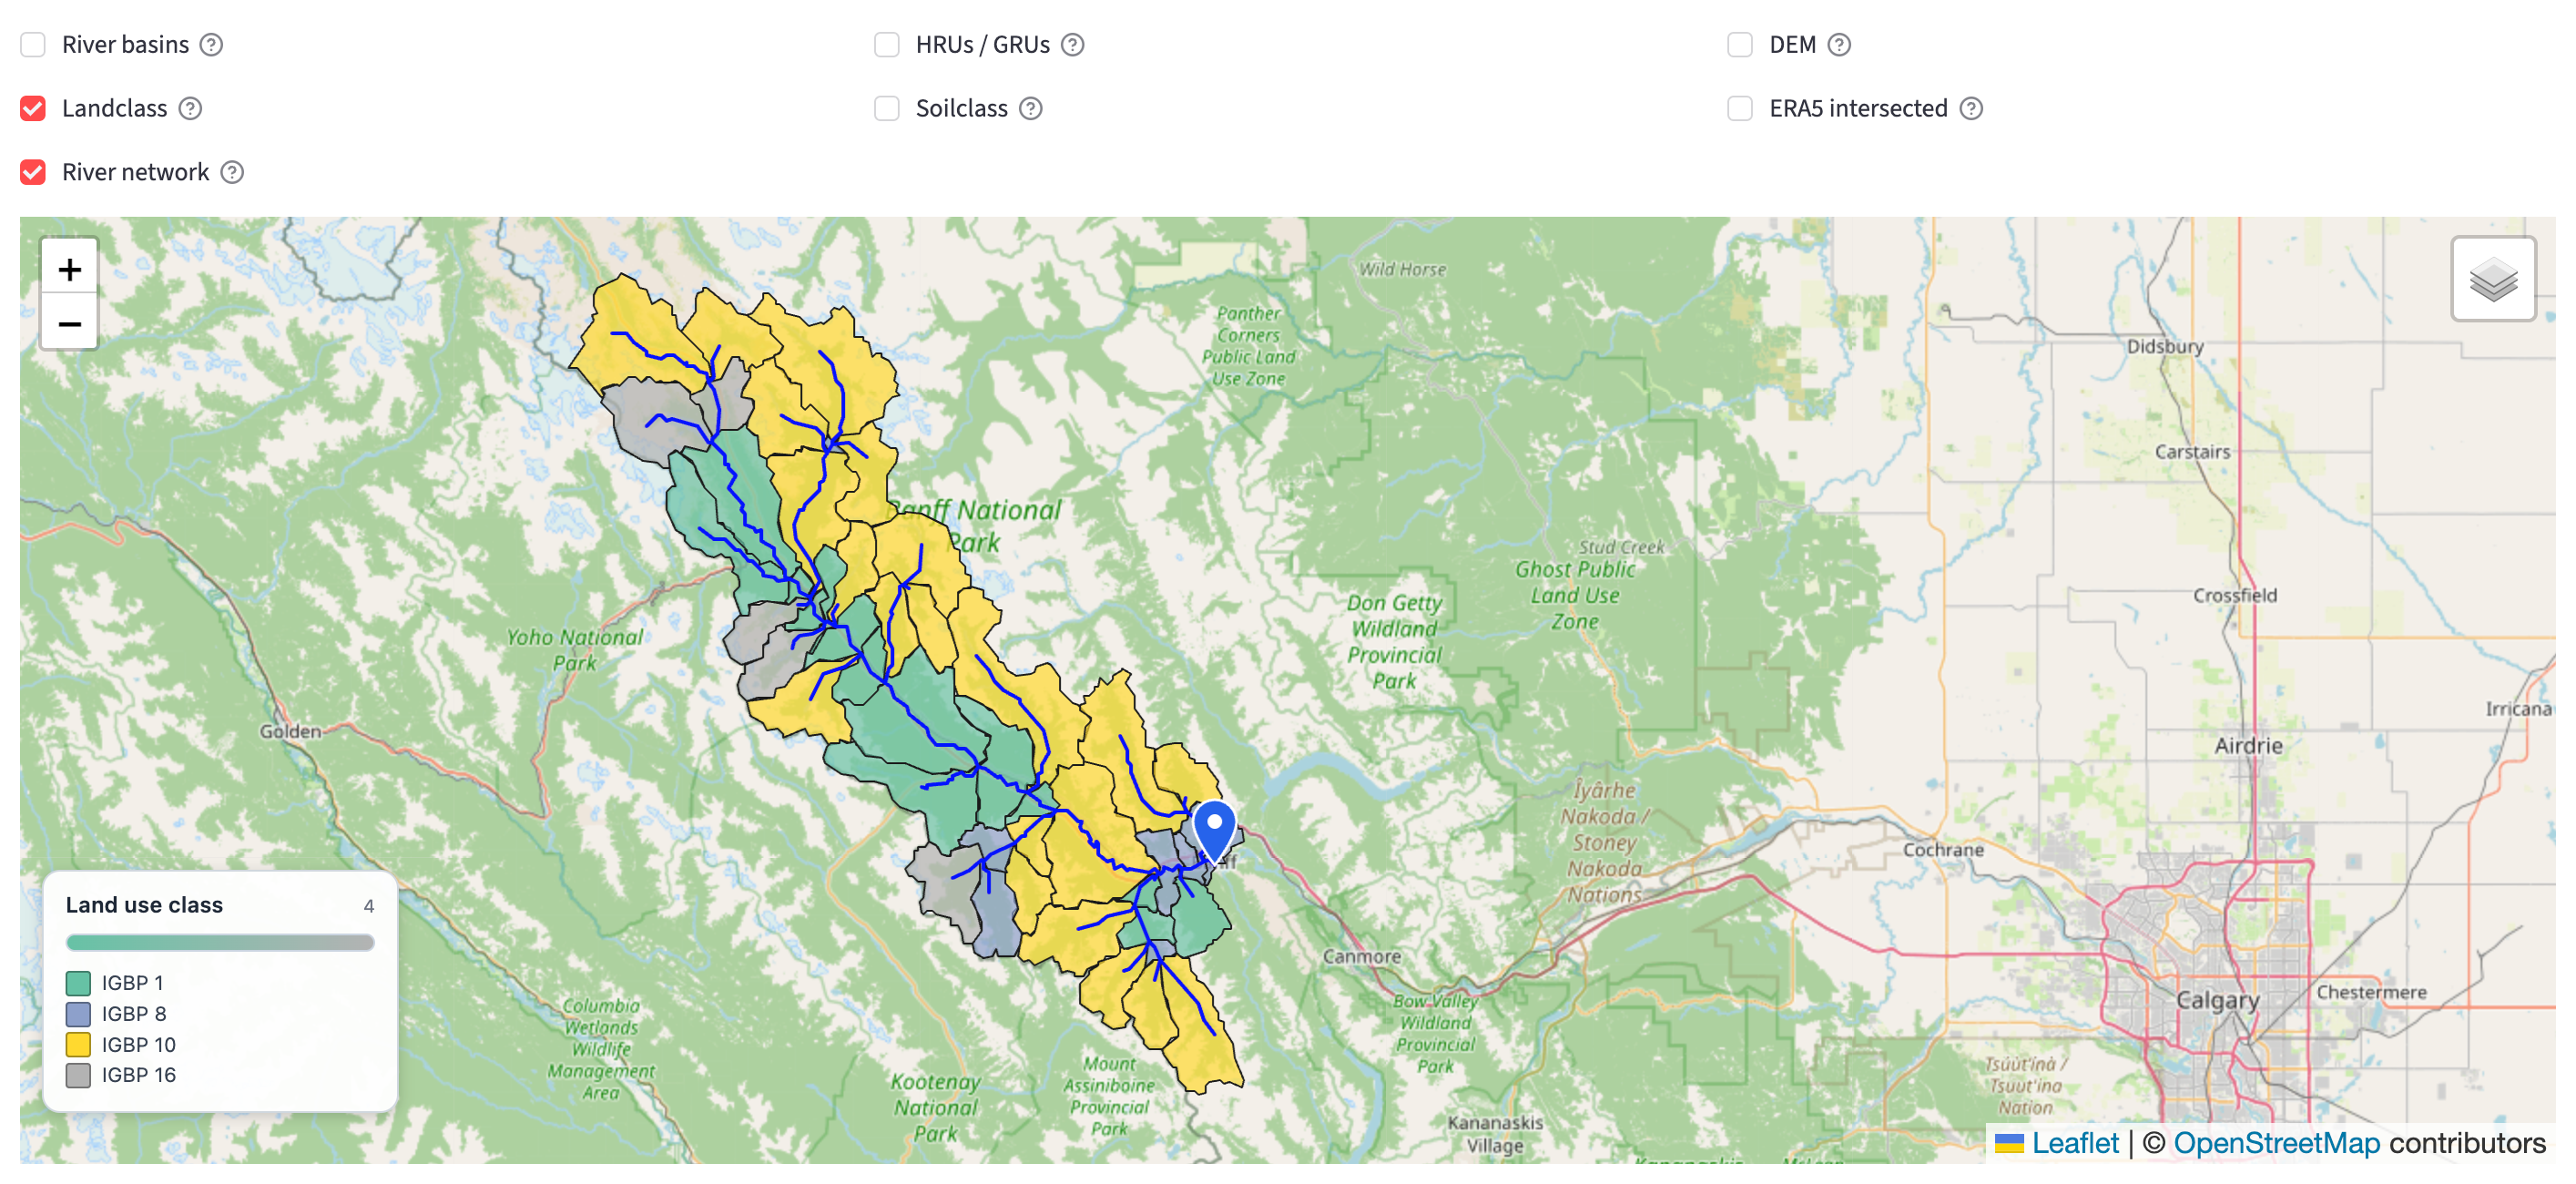
\includegraphics[width=\textwidth]{figs/land_classes.png}
  \caption{Land-use classes generated for the Bow River at Banff semi-distributed case study. 
  The map shows the spatial distribution of land-use categories across the delineated modelling 
  units, together with the river network and pour point used in the workflow.}
  \label{fig:land-classes}
\end{figure}

\begin{figure}[!t]
  \centering
  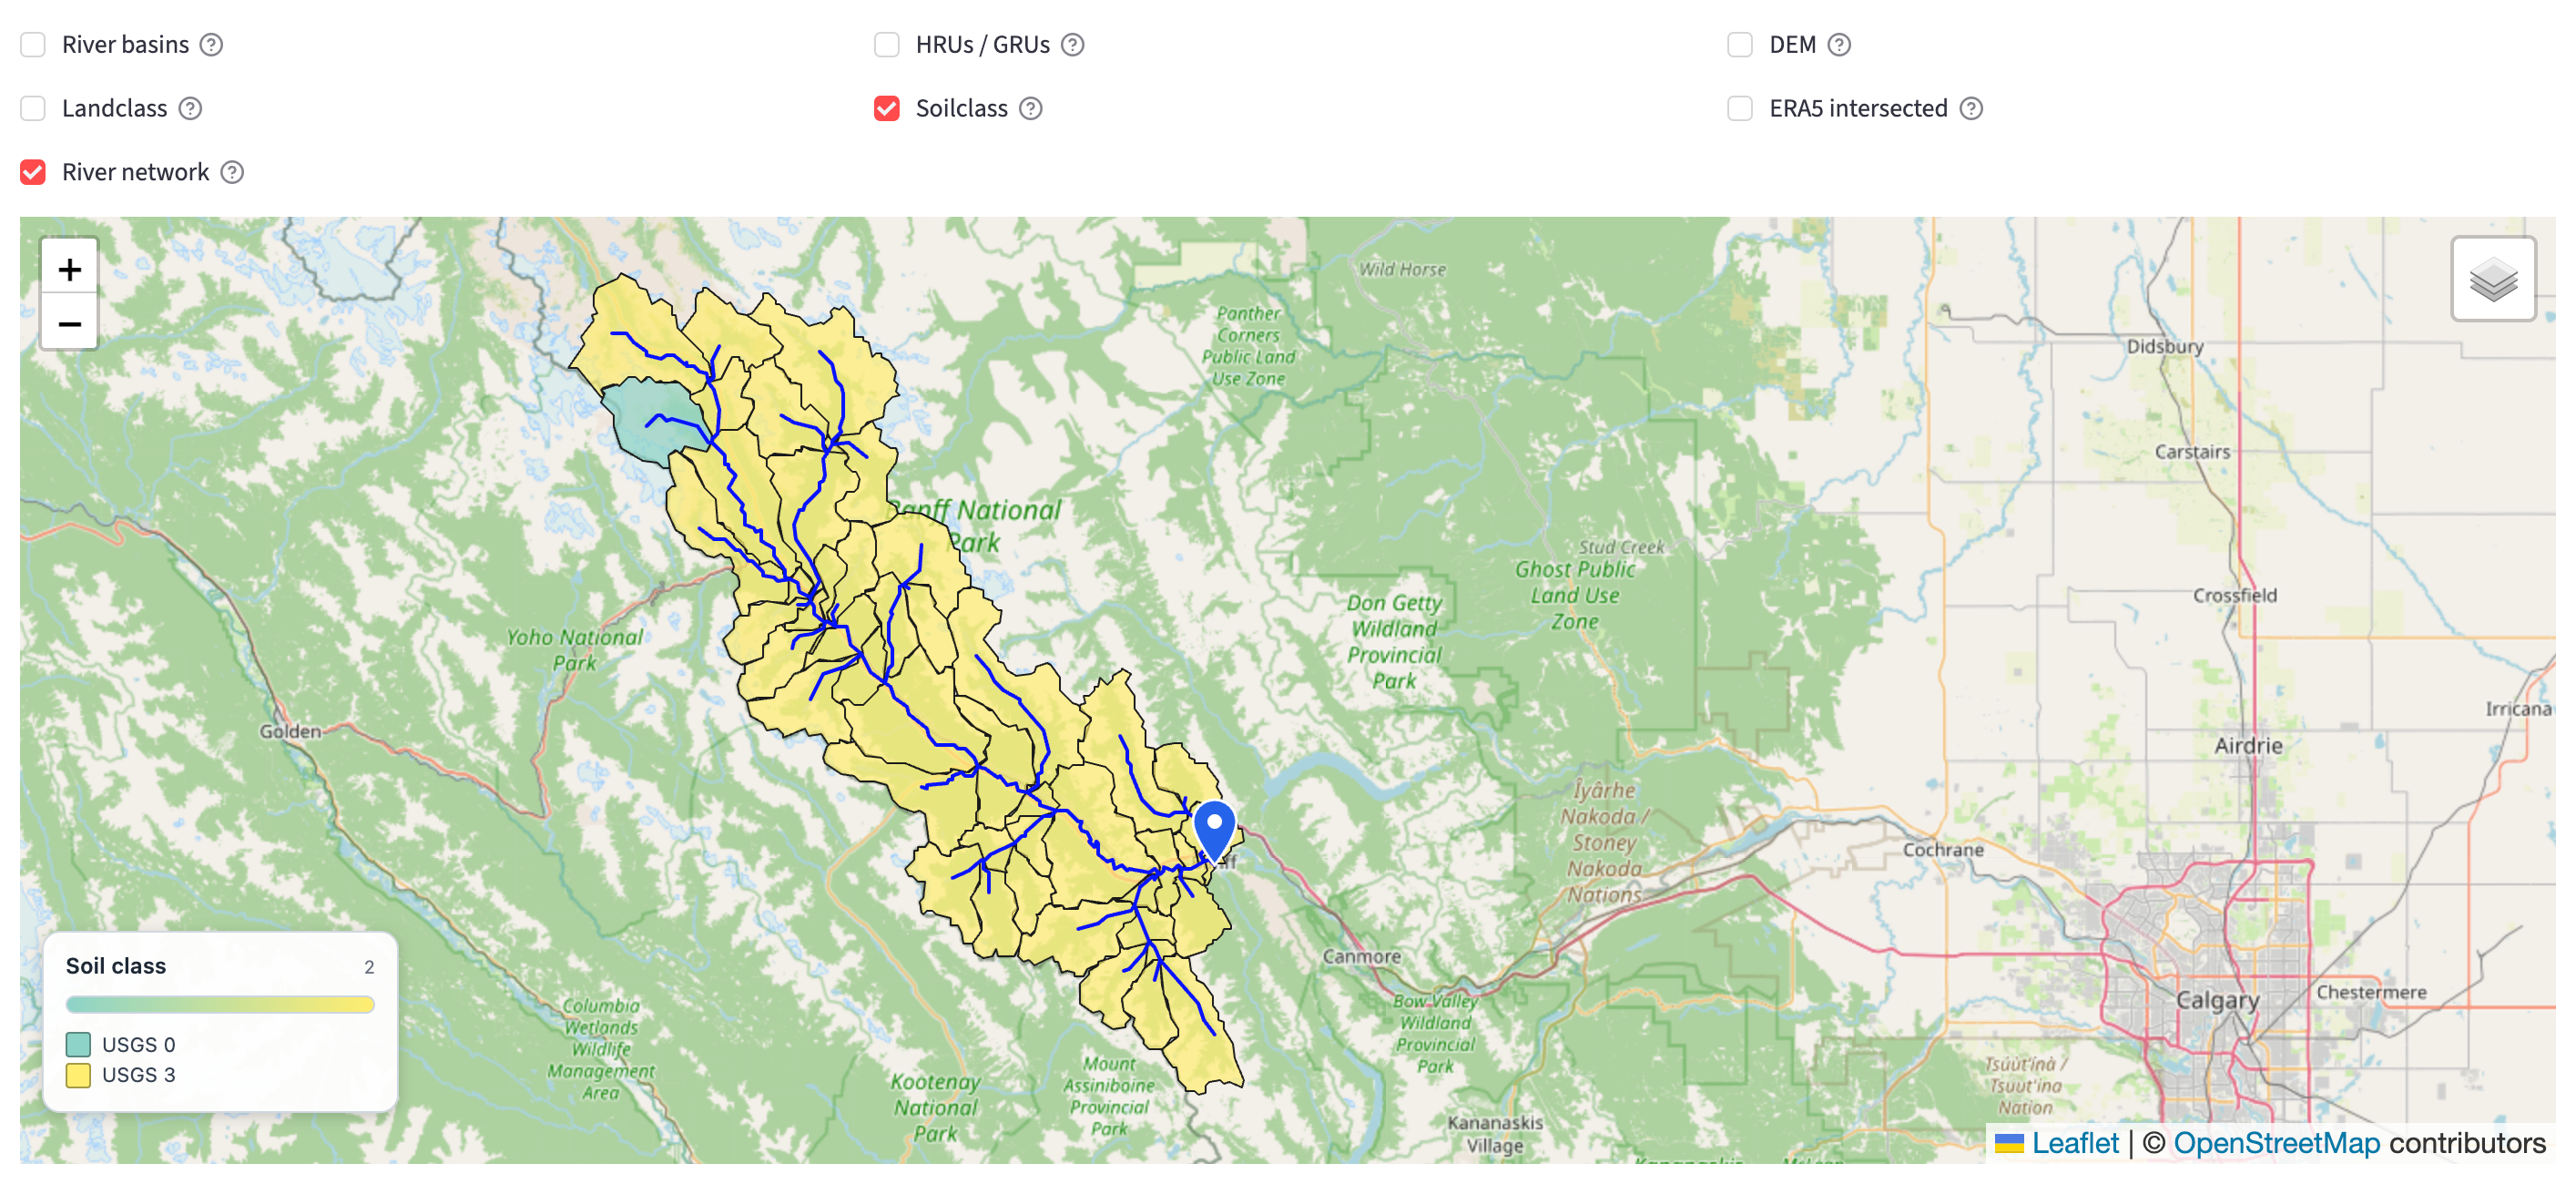
\includegraphics[width=\textwidth]{figs/soil_classes.png}
  \caption{Soil classes generated for the Bow River at Banff semi-distributed case study. The 
  map shows the spatial distribution of soil categories across the delineated modelling units, 
  together with the river network and pour point used in the workflow.}
  \label{fig:soil-classes}
\end{figure}


\subsection{Case study 2: Bow River at Banff lumped SUMMA workflow}

The second case study evaluated HydroAgent on a simpler lumped Bow River at Banff workflow. The 
prompt requested a lumped SUMMA setup using the domain name \texttt{Bow\_at\_Banff\_lumped}, 
experiment identifier \texttt{run\_1}, pour point \texttt{51.1722/-115.5717}, WSC station 
identifier \texttt{05BB001}, ERA5 forcing, cloud data access, stream-threshold delineation, 
and the 2004--2007 experiment period. The prompt also explicitly requested that \texttt{mizuRoute} 
not be used for this lumped case.

HydroAgent extracted the expected configuration fields, including the domain name, experiment 
identifier, pour point, WSC station identifier, hydrological model \texttt{SUMMA}, forcing 
dataset \texttt{ERA5}, data-access mode \texttt{cloud}, stream-threshold value \texttt{5000}, 
lumped discretization, spinup period \texttt{2004-01-01, 2005-09-30}, calibration period 
\texttt{2005-10-01, 2006-09-30}, and evaluation period \texttt{2006-10-01, 2007-12-30}. The 
generated workflow followed the expected step order exactly, using the same ordered sequence 
shown in Listing~\ref{lst:semidistributed-steps}. No step reordering was required.

The run produced the expected HydroAgent provenance artifacts, including \texttt{prompt.txt}, 
\texttt{plan.json}, \texttt{spec.json}, \texttt{config.yaml}, \texttt{chat.json}, \texttt{workflow\_job.json}, 
and \texttt{logs/execution.log}. All executed workflow steps completed successfully with return 
code 0. SUMMA produced non-empty timestep and daily output files: \texttt{run\_1\_timestep.nc} 
contained 35,063 time records, and \texttt{run\_1\_day.nc} contained 1,460 daily records.

The reporting outputs included \path{domain_map.png}, \path{domain_discretization_GRUs.png}, 
\path{run_1_comparison_overview.png}, and \path{run_1_default_vs_calibrated.png}.

Although the original prompt requested a lumped SUMMA workflow without \texttt{mizuRoute}, 
the generated plan retained \texttt{mizuRoute} as the routing model, and the backend 
dependency logic automatically added \texttt{MIZUROUTE} as a dependency of \texttt{SUMMA}. 
The execution log reported that both the SUMMA run and the mizuRoute run completed successfully. 
This case is therefore reported as a lumped SUMMA workflow with automatically added routing, 
rather than as a pure SUMMA-only run. The result highlights the importance of inspecting the 
generated plan and execution log even when the natural-language prompt explicitly excludes a 
workflow component.

\subsection{Case study 3: Local artifact reuse and missing-file recovery}

The third case study evaluated HydroAgent's ability to support recovery-oriented modelling 
when a partially prepared local domain already exists. This case reused the semi-distributed 
Bow River at Banff domain created in Case Study 1, but executed a new experiment, 
\texttt{run\_local\_recovery\_1}. The purpose was to test whether HydroAgent could preserve 
the original hydrological domain name, avoid unnecessary cloud data acquisition, reuse local 
artifacts, regenerate stale or missing preprocessing files, and complete model execution 
without rebuilding the entire workflow from scratch.

The prompt explicitly instructed HydroAgent to reuse the existing local workspace, 
\path{SYMFLUENCE_data/domain_Bow_at_Banff_semi_distributed}, and to preserve 
\texttt{domain\_name = Bow\_at\_Banff\_semi\_distributed}. It also instructed the agent 
not to create suffixed domain folders, such as \path{domain_Bow_at_Banff_semi_distributed (1)}. 
The same prompt specified \texttt{experiment\_id = run\_local\_recovery\_1}, pour point 
\texttt{51.1722/-115.5717}, WSC station \texttt{05BB001}, ERA5 forcing, SUMMA with mizuRoute 
routing, GRU discretization, and the same 2004--2007 experiment period used in Case Study 1. 
The generated plan set local data access and removed unnecessary acquisition steps when the 
required local artifacts were available.

HydroAgent executed \texttt{setup\_project} and \texttt{create\_pour\_point} in the existing 
domain, then completed \texttt{model\_agnostic\_preprocessing}. The workflow reused the local 
ERA5 forcing files and did not repeat the long cloud-forcing download. During model-specific 
preprocessing, HydroAgent processed 48 ERA5 forcing files, removed stale SUMMA forcing files, 
regenerated temperature-lapsed SUMMA inputs, recreated the SUMMA forcing-file list, file 
manager, attributes file, cold-state file, trial-parameter file, and mizuRoute topology file. 
SUMMA then executed successfully, followed by mizuRoute, which used the generated SUMMA timestep 
runoff file.

The run completed \texttt{postprocess\_results} and produced \path{results/run_local_recovery_1_results.csv} 
and \path{data/model_output/run_local_recovery_1_results.nc}. It demonstrates workflow 
robustness: HydroAgent maintained domain identity, reused local artifacts, regenerated required 
model inputs, and completed SUMMA--mizuRoute execution in a local-recovery setting.

\subsection{Case study 4: Conversational workflow refinement}

The fourth case study evaluated HydroAgent's ability to revise a structured workflow plan through 
multi-turn conversation. Unlike Case Study 3, which tested execution of a local-recovery workflow, 
this case focused on the planning and refinement stage before model execution. Starting from an 
initial Bow River at Banff SUMMA request, the user progressively modified the generated plan by 
adding a \texttt{bounding box}, changing the \texttt{experiment\_ id}, switching the \texttt{forcing\_data} mode, 
specifying a semi-distributed GRU workflow with mizuRoute routing, defining \texttt{spinup}, \texttt{calibration}, 
and \texttt{evaluation} periods, removing \texttt{acquire\_forcings} from the execution steps, and 
adding \texttt{postprocess\_results}. After each message, HydroAgent updated the 
persistent \texttt{plan.json} representation and reported the corresponding plan changes 
to the user.

Figure~\ref{fig:case4-refinement} shows the chat interaction and the associated changes 
in \texttt{plan.json}. The purpose of this case was not to demonstrate another completed 
model run, but to show that conversation acts as a controlled editing layer over a structured 
workflow plan. This capability is important because users often refine hydrological experiments 
incrementally, and the agent must preserve consistency across configuration fields, workflow 
steps, and execution constraints as the plan evolves.

\begin{figure}[!t]
  \centering
  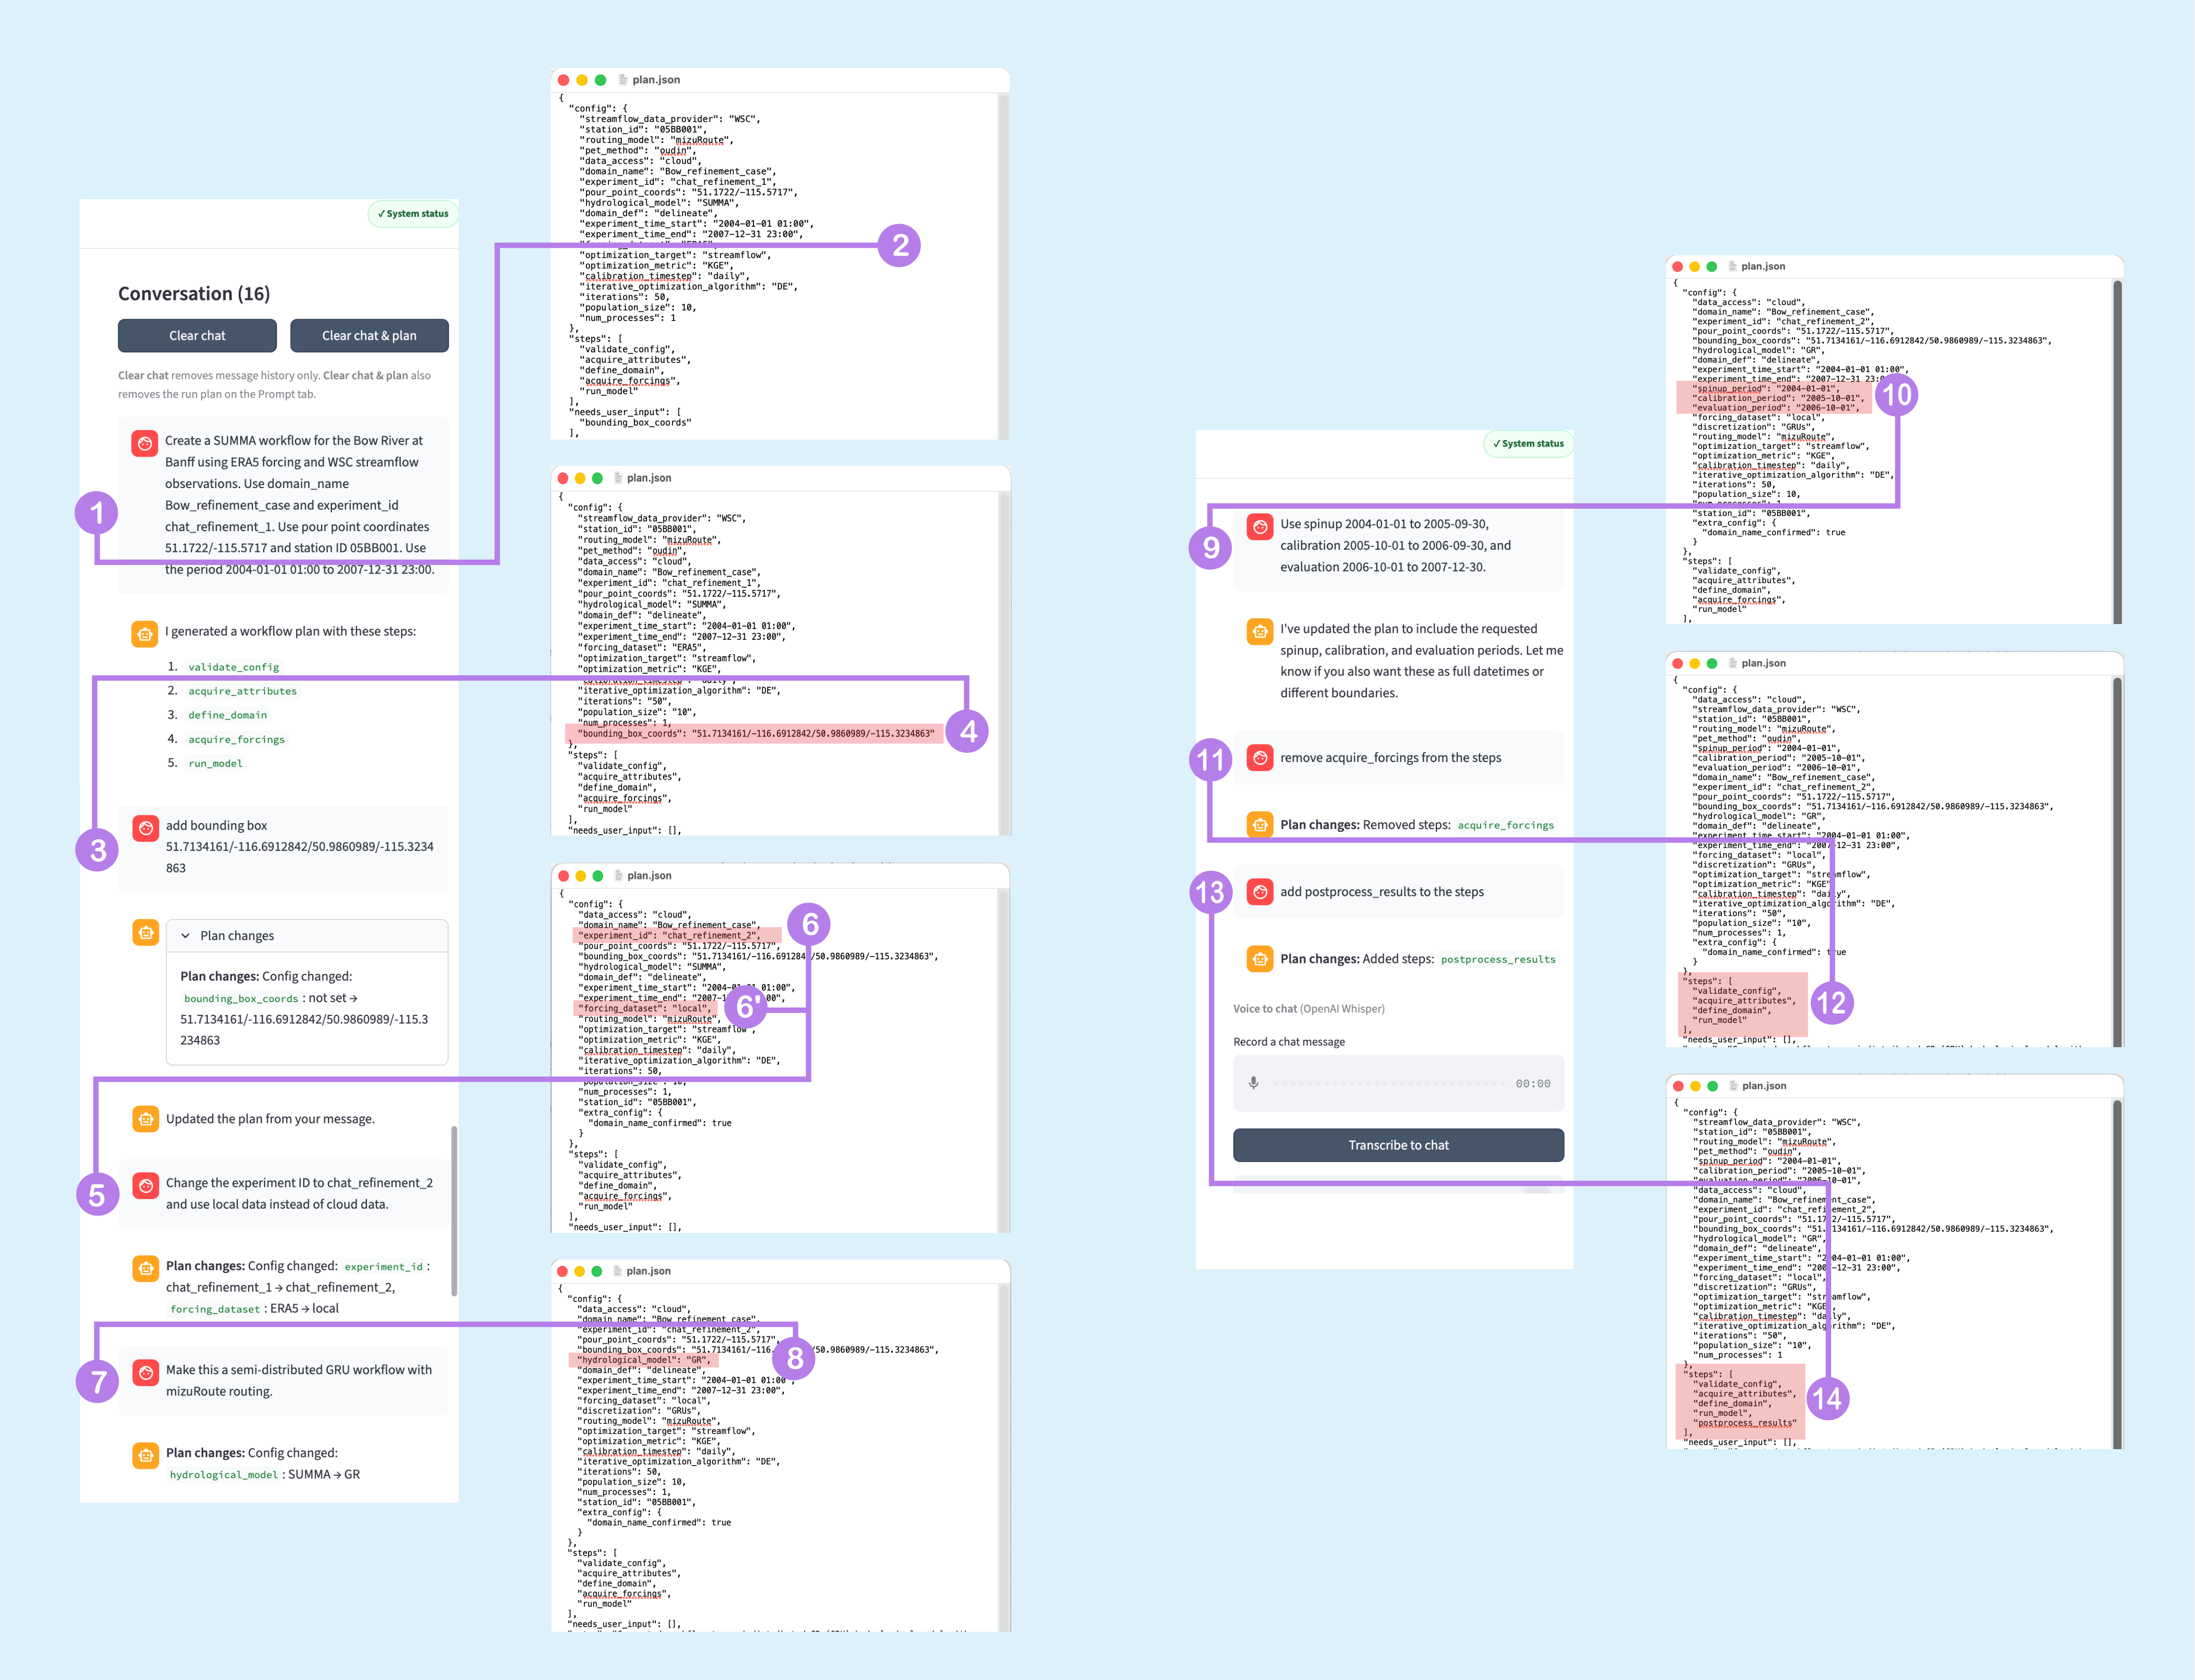
\includegraphics[width=\textwidth]{figs/case4.png}
  \caption{Conversational workflow refinement in HydroAgent. The user begins with a 
  natural-language Bow River at Banff modelling request, after which HydroAgent generates 
  an initial structured plan. Subsequent chat messages refine the workflow by adding a 
  bounding box, changing the experiment identifier and forcing data mode, switching to a 
  semi-distributed GRU workflow with mizuRoute routing, defining spinup, calibration, and 
  evaluation periods, removing forcing acquisition from the execution steps, and adding 
  postprocessing. The highlighted \texttt{plan.json} panels show that chat refinements 
  update the structured workflow plan rather than only generating free-text responses.}  
  \label{fig:case4-refinement}
\end{figure}


% ============================================================
\section{Evaluation}
\label{sec:evaluation}
% ============================================================

The evaluation examines HydroAgent as a workflow-planning and execution-control system 
rather than as a hydrological model calibration system. The goal is to determine whether 
natural-language requests can be converted into structured, inspectable, and backend-compatible 
workflow plans, and whether those plans can be validated, refined, and executed safely. The 
evaluation therefore focuses on prompt-to-plan alignment, provider behavior, missing-input 
handling, negative-constraint compliance, local-versus-cloud intent, conversational refinement, 
and workflow execution outcomes.

\subsection{Prompt-to-plan evaluation}

A prompt-to-plan evaluation was conducted using 25 natural-language hydrological workflow 
prompts. The prompts were designed to cover common and challenging HydroAgent use cases, 
including full SUMMA workflows, semi-distributed GRU workflows, lumped workflows, 
elevation-distributed workflows, local-data reuse, cloud-data acquisition, calibration 
requests, explicit step-list requests, dry-run-only requests, missing-input cases, and 
negative constraints such as \texttt{do not run the model}, \texttt{do not calibrate}, 
\texttt{do not download attributes or forcings}, and \texttt{do not use mizuRoute}. For 
each prompt, the generated \texttt{plan.json} was inspected for three properties: (i) 
whether the requested configuration fields were extracted correctly, (ii) whether the 
workflow steps matched the user request and the expected backend dependencies, and 
(iii) whether missing inputs or unsafe execution conditions were represented through 
\texttt{needs\_user\_input} or \texttt{dry\_run} behavior.

Across the prompt set, HydroAgent performed strongest on configuration extraction and 
missing-input detection. The generated plans generally captured domain names, experiment 
identifiers, pour-point coordinates, hydrological model names, forcing datasets, time 
windows, discretization choices, calibration and evaluation periods, optimization metrics, 
and iteration counts. Under-specified prompts were usually handled conservatively by 
returning \texttt{validate\_config} or \texttt{dry\_run} plans and listing missing fields 
such as \texttt{domain\_name}, \texttt{pour\_point\_coords}, \texttt{bounding\_box\_coords}, 
or experiment dates in \texttt{needs\_user\_input}. This behavior is important because it 
prevents incomplete natural-language requests from being converted directly into expensive 
backend operations.

The main weakness was workflow-step alignment. Several plans extracted the correct 
configuration fields but produced incomplete or overly broad step lists. Some executable 
workflows included \texttt{run\_model} while omitting one or more prerequisite steps, such 
as \texttt{setup\_project}, \texttt{create\_pour\_point}, \texttt{acquire\_forcings}, 
\texttt{model\_agnostic\_preprocessing}, or \texttt{model\_specific\_preprocessing}. In 
other cases, restricted prompts were expanded into broader workflows than requested. 
These results support the hybrid design of HydroAgent: the LLM-generated plan should be 
treated as a structured draft that becomes executable only after deterministic validation, 
dependency repair, and user confirmation.

\begin{table}[H]
\centering
\small
\caption{Summary of prompt-to-plan evaluation results from the 25-prompt test set.}
\label{tab:prompt-plan-evaluation}
\begin{tabularx}{\textwidth}{P{0.27\textwidth} Z Z}
\toprule
\textbf{Evaluation aspect} & \textbf{Observed strength} & \textbf{Observed limitation} \\
\midrule

Configuration extraction
& Core fields such as \texttt{domain\_name}, \texttt{experiment\_id}, \texttt{pour\_point\_coords}, \texttt{hydrological\_model}, \texttt{forcing\_dataset}, dates, calibration periods, and optimization settings were generally extracted correctly.
& Some specialized settings were inconsistently represented, appearing in \texttt{extra\_config} or notes rather than as standardized first-class fields. \\

Missing-input handling
& Under-specified prompts were usually converted to safe validation or dry-run plans, with missing fields listed in \texttt{needs\_user\_input}.
& In some cases, planner notes and configuration fields were inconsistent about which inputs were missing. \\

Workflow-step selection
& Explicit dry-run, validation-only, and no-run requests were often respected, and user-specified step lists were often preserved.
& Some executable workflows omitted prerequisite steps, while some restricted prompts were expanded into broader workflows than requested. \\

Negative constraints
& Instructions such as ``do not run the model'', ``do not calibrate'', and ``do not download attributes or forcings'' were often reflected in the generated step list.
& Negative constraints require validation after backend dependency resolution because omitted components can be reintroduced by backend rules. \\

Local-versus-cloud intent
& Local-reuse prompts generally avoided cloud acquisition steps, and cloud prompts generally included acquisition steps.
& Some local-reuse plans still included unnecessary domain-definition or preprocessing steps, and local-data intent was not always encoded consistently. \\

Planner transparency
& Notes often explained extracted fields, inferred defaults, missing inputs, and step decisions.
& Notes were sometimes overly verbose or contradictory, especially when the step list and \texttt{needs\_user\_input} did not fully agree. \\

\bottomrule
\end{tabularx}
\end{table}

\subsection{Provider comparison}

The same 25-prompt evaluation set was run using three LLM providers: OpenAI, Google Gemini, 
and Anthropic Claude. The comparison was limited to plan generation. Backend hydrological 
execution was not repeated for every provider because HydroAgent normalizes the generated 
\texttt{plan.json} before passing it to the SYMFLUENCE adapter. Once a plan is validated 
and repaired, the backend receives the same structured representation regardless of which 
provider generated the initial draft.

All three providers were able to produce usable structured plans for most prompts, and all 
three generally extracted core fields correctly. However, the providers showed different 
planning tendencies. OpenAI was the most conservative provider: it more consistently 
respected restricted prompts such as \texttt{dry\_run}, "do not run the model", 
and "do not use \texttt{mizuRoute}". Gemini often produced richer configuration objects 
and more frequently preserved specialized settings such as discretization and elevation-band 
size, but it sometimes requested unnecessary inputs or expanded the workflow beyond the 
user's requested scope. Claude produced detailed plans and often included complete workflow 
sequences, but it was also the most likely to over-expand limited requests into broader 
execution workflows.

\begin{table}[H]
\centering
\small
\caption{Qualitative comparison of OpenAI, Gemini, and Claude on the 25-prompt planning evaluation.}
\label{tab:provider-comparison}
\begin{tabularx}{\textwidth}{P{0.20\textwidth} Z Z Z}
\toprule
\textbf{Evaluation aspect} & \textbf{OpenAI} & \textbf{Gemini} & \textbf{Claude} \\
\midrule

Core field extraction
& Correctly extracted most domain names, experiment identifiers, pour points, dates, model names, and forcing datasets.
& Correctly extracted most core fields and often added additional defaults such as discretization.
& Correctly extracted most core fields and often produced detailed configuration objects. \\

Missing-input handling
& Generally conservative; missing fields were usually reflected in \texttt{needs\_user\_input} or \texttt{dry\_run}.
& Usually detected missing inputs, but sometimes requested additional inputs for limited workflows.
& Usually detected missing inputs, but notes sometimes contradicted the actual extracted fields. \\

Negative constraints
& Most consistently respected instructions such as ``do not run the model'', ``do not calibrate'', and ``do not use \texttt{mizuRoute}''.
& Often respected negative constraints, but sometimes expanded the workflow beyond the requested scope.
& Sometimes respected omitted components, but often retained broad execution workflows even for restricted prompts. \\

Specialized configuration
& Sometimes omitted specialized settings from explicit configuration fields.
& Often preserved specialized settings such as \texttt{discretization} and \texttt{ELEVATION\_BAND\_SIZE}.
& Often preserved specialized settings and produced detailed explanatory notes. \\

Workflow-step alignment
& More conservative and safer for dry-run prompts, but sometimes under-included preprocessing steps for executable workflows.
& Balanced in many cases, but sometimes over-expanded or requested unnecessary prerequisites.
& Often produced complete full-workflow sequences, but sometimes over-expanded limited requests. \\

Overall tendency
& Conservative and safety-oriented.
& Configuration-rich but sometimes over-specific.
& Detailed and expansive, but sometimes too broad. \\

\bottomrule
\end{tabularx}
\end{table}

The provider comparison supports HydroAgent's provider-agnostic architecture. No provider 
produced uniformly perfect plans, but all three produced useful structured drafts. The 
value of HydroAgent therefore lies not in assuming that one LLM is always correct, but in 
placing provider outputs behind a shared schema, deterministic normalization, operation-catalog 
validation, dependency repair, and explicit execution gates.

\subsection{Negative constraints and safety behavior}

A subset of prompts tested whether HydroAgent respected explicit negative constraints. 
These included instructions not to run the model, not to calibrate, not to download 
attributes or forcings, and not to use mizuRoute. The initial plans often represented 
these constraints correctly by omitting forbidden steps such as \texttt{run\_model}, 
\texttt{calibrate\_model}, \texttt{acquire\_attributes}, or \texttt{acquire\_forcings}. 
However, the evaluation also shows that negative constraints must be checked after 
backend dependency resolution. In the lumped Bow River case study, the prompt requested 
a SUMMA-only workflow without mizuRoute, but routing was retained and executed as a 
backend dependency. This limitation demonstrates why the final plan, resolved dependency 
list, and execution log must remain visible to the user before and after execution.

\subsection{Case-study execution evaluation}

The prompt-to-plan and provider-comparison experiments evaluated planning behavior. The case studies evaluated whether generated and refined plans could support realistic HydroAgent workflows with the SYMFLUENCE backend. Case Study 1 demonstrated end-to-end execution of a cloud-from-scratch semi-distributed SUMMA--mizuRoute workflow. The run produced the expected run-level provenance artifacts, non-empty SUMMA timestep and daily outputs, a mizuRoute output file, and reporting figures. Case Study 2 demonstrated successful execution of a simpler lumped workflow, while also exposing the negative-constraint limitation in which mizuRoute was retained despite the prompt requesting a SUMMA-only workflow. Case Study 3 demonstrated local-artifact reuse and missing-file recovery by preserving the original hydrological domain name, avoiding unnecessary cloud forcing acquisition, regenerating stale preprocessing and model-specific files, running SUMMA and mizuRoute, and producing postprocessed CSV and NetCDF outputs. Case Study 4 demonstrated multi-turn conversational refinement of a persistent \texttt{plan.json}, showing that chat updates structured workflow state rather than only producing free-text responses.

\begin{table}[H]
\centering
\small
\caption{Execution and refinement outcomes from the four HydroAgent case studies.}
\label{tab:case-execution-evaluation}
\begin{tabularx}{\textwidth}{P{0.23\textwidth} Z Z}
\toprule
\textbf{Case study} & \textbf{Evaluation focus} & \textbf{Outcome} \\
\midrule

Semi-distributed SUMMA + \texttt{mizuRoute}
& End-to-end cloud-from-scratch execution.
& Completed workflow with provenance artifacts, SUMMA timestep and daily outputs, 
\texttt{mizuRoute} output, and reporting figures. \\

Lumped SUMMA with automatically added routing
& Simpler workflow execution and dependency transparency.
& Completed execution and produced non-empty SUMMA outputs, but exposed a limitation 
because \texttt{mizuRoute} was retained despite a no-routing prompt. \\

Local artifact reuse and missing-file recovery
& Local-data reuse, domain-name preservation, and recovery from stale or missing artifacts.
& Preserved the original hydrological domain, reused local artifacts, regenerated required 
preprocessing/model files, completed SUMMA--\texttt{mizuRoute} execution, and produced postprocessed 
outputs. \\

Conversational workflow refinement
& Multi-turn editing of a persistent structured plan.
& Updated \texttt{plan.json} across chat turns as the user modified bounding box, experiment 
identifier, data-access mode, routing, time periods, and execution steps. \\

\bottomrule
\end{tabularx}
\end{table}

\subsection{Limitations of the evaluation}

The current evaluation is intentionally practical and case-study based. It demonstrates 
feasibility, planning behavior, provider differences, execution success, local-artifact reuse, 
and conversational refinement, but it is not yet a large formal benchmark across many basins, 
users, hydrological models, or backend frameworks. The 25-prompt evaluation was manually 
inspected rather than scored by multiple independent annotators. The provider comparison was 
qualitative rather than a statistically powered benchmark, and backend execution was not 
repeated for every provider. Future work should expand this evaluation into a larger benchmark 
with expert reference plans, inter-rater agreement, repeated trials, automatic scoring of field 
accuracy and step alignment, additional basins, additional users, and additional backend adapters.

% ============================================================
\section*{Competing interests}

The author declares no competing interests.

\section*{Acknowledgements}




\bibliographystyle{plainnat}
\bibliography{references}

\end{document}


